% !TeX spellcheck = ru_RU
\section{Эталонные модели сетевого взаимодействия}
Существуют две основные модели, описывающие взаимодействие устройств в компьютерных сетях.
\begin{itemize}
	\item OSI (содержит 7 уровней)
	\item TCP/IP (содержит 4 уровней)
\end{itemize}
\begin{table}[h!]
	\centering
	\begin{tabular}{|l|l|l|l|}
		\hline
			\multicolumn{2}{|c|}{Уровень} & \multicolumn{1}{c|}{Функции} & \multicolumn{1}{c|}{Примеры протоколов} \\ \hline
			7 & Приложения & Протоколы пользовательских приложений & HTTP(S), POP3, SMTP \\ \hline
			6 & Представления & Сжимание, шифрование &  \\ \hline
			5 & Сессионный & Контроль сессии &  \\ \hline
			4 & Транспортный &  & UDP, TCP \\ \hline
			3 & Сетевой & Протоколы глобального взаимодействия & IPv4, IPv6 \\ \hline
			2 & Канальный & Протоколы локального взаимодействия & Ethernet (MAC) \\ \hline
			1 & Физический & Кабели, коннекторы & Ethernet (PHY) \\ \hline
	\end{tabular}
	\caption{Структура модели OSI}
	\label{tbl:osi}
\end{table}
Структура первой модели представлена в таблице~\ref{tbl:osi} вместе с примерами протоколов, работающих на разных уровнях. Все сетевые устройства работают на различных уровнях (стоит отметить, что существуют устройства, затрагивающие сразу несколько уровней). Вот несколько примеров:
\begin{itemize}
	\item физический --- концентраторы, повторители, медиаконвертеры;
	\item канальный --- мосты, коммутаторы
	\item сетевой --- маршрутизаторы (роутеры)
	\item транспортный --- шлюзы и брандмауэры
\end{itemize}
Некоторые из этих устройств будут подробно рассмотрены позже.
\section{Инкапсуляция и декапсуляция}
\begin{figure}[h!]
	\centering
	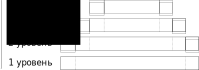
\includegraphics[width=0.8\linewidth]{pic/incapsulation.pdf}
	\caption{Процесс инкапсуляции}
	\label{fig:incapsulation}
\end{figure}
Рассмотрим подробнее схему передачи данных в компьютерных сетях. (см. рис.~\ref{fig:incapsulation}). Когда на уровень приложений поступают данные для передачи, протокол 7 уровня добавляет к данным какой-то свой заголовок и концевик (необязательно) и передает полученный блок данных на уровень ниже. Далее процесс повторяется, пока пакет не дойдет до физического уровня, когда, собственно, начнется передача данных. Во время приема данных происходит обратный процесс --- декапсуляция. 

Важно конкретно называть блоки данных (Protocol Data Unit, PDU), которыми оперируют разные уровни модели OSI. Так, в частности:
\begin{itemize}
	\item 1 уровень --- бит;
	\item 2 уровень --- кадр;
	\item 3 уровень --- пакет;
	\item 4 уровень --- сегмент.
\end{itemize}

Стоит отметить, что каждое устройство производит инкапсуляцию и декапсуляцию лишь до того уровня на котором оно работает (см. рис~\ref{fig:incapsulation_devices}).
\begin{figure}[h!]
	\centering
	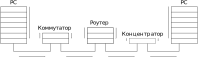
\includegraphics[width=0.8\linewidth]{pic/incapsulation_devices.pdf}
	\caption{Инкапсуляция и декапсуляция на различных устройствах}
	\label{fig:incapsulation_devices}
\end{figure}

\section{Литература}
\begin{itemize}
	\item ICND1 \cite{icnd1eng}, Глава 1.
\end{itemize}